
\chapter{Uncomplicated Statistical \hnmr{} NMR Spectral Remodeling}

\section{Introduction}

\begin{doublespace}
Structure-activity relationships (SAR) by NMR \cite{shuker:sci1996} spurred
a revolution for the role of NMR in drug discovery. Like X-ray crystallography,
NMR had been primarily used as a means to determine protein and protein-ligand
structures as part of a structure-based drug discovery effort
\cite{ferentz:qrb2000}. NMR is now an important alternative to traditional
high-throughput screening (HTS) assays for identifying drug-like chemical
leads \cite{pellecchia:nrdd2002,powers:eodd2009}. By combining NMR
ligand-affinity screens with fragment-based libraries, a dramatic increase in
chemical diversity is achieved (from $10^6$ to $10^{63}$), while also
minimizing resources, increasing hit-rates and improving the drug-like
qualities of the resulting chemical leads \cite{hajduk:nrdd2007}. Consequently,
NMR fragment-based screens have significantly benefited the pharmaceutical
industry by leading to a number of clinical-stage compounds.
\\\\
NMR ligand-affinity screening is also a powerful platform for protein
functional annotation during the search for novel drug targets
\cite{mercier:cchts2009,powers:ddt2008}. Significant percentages of the human
proteome and the proteomes of other infectious organisms are comprised of
functionally uncharacterized proteins \cite{muller:genres2002}. Undoubtedly
hidden among this multitude of unannotated proteins are novel drug targets
that may lead to new treatments or new means of overcoming mechanisms of drug
resistance. Besides verifying that a functionally unannotated protein is
druggable, NMR ligand affinity screening also identifies the functional
epitope and the classes of ligands that bind the uncharacterized protein.
This information may then be leveraged to infer a function through structural
similarities with functionally annotated proteins
\cite{powers:prot2006,powers:bmcrn2011}.
\\\\
NMR spectroscopy reports a multitude of time-averaged physical observables
that carry information relating to the nature of interactions between small
molecule ligands and protein targets \cite{lepre:chemrev2004}. A number of
1D \hnmr{} NMR pulse sequences have been developed to probe these distinct
features of binding, including differences in free and bound ligand diffusion
and relaxation properties \cite{hajduk:jacs1997}, and saturation transfers
from water \cite{dalvit:jbnmr2000} and protein \cite{mayer:jacs2001}
resonances. As part of an NMR high-throughput screen, these 1D \hnmr{} NMR
pulse sequences present a number of unique challenges that include high false
positive rates, long acquisition times, and high demand for protein samples
\cite{lepre:menz2011,harner:jbnmr2013}. However, at suitably chosen
concentrations of ligand and protein, a standard, unedited 1D \hnmr{} NMR
experiment may be used to detect binding interactions through enhanced
relaxation rates of ligand spins
\cite{mercier:jacs2006,powers:ddt2008,mercier:cchts2009}.
\\\\
While it is possible to detect ligand binding using standard 1D \hnmr{} NMR,
the resulting spectra are a combination of free and bound ligand and protein
signals, a fact which makes them difficult to interpret. Broad, rolling
baselines arising from slowly tumbling protein spins are particularly
problematic during interpretation, as they often mask changes in ligand signal
broadness and intensity. This masking effect due to protein baselines is
exacerbated at protein-ligand concentration ratios nearing or exceeding unity,
forcing the use of excess ligand and increasing the false negative rate during
screening. To mitigate these issues, a statistical method called Uncomplicated
Statistical Spectral Remodeling (USSR), was developed that removes protein
baselines from high-throughput ligand-based screening datasets by leveraging
inter-sample reproducibility of protein signals. In addition, it will be
demonstrated that the use of phase-scatter correction greatly improves
inter-sample protein baseline reproducibility and reduces the false-positive
rate incurred by subsequent USSR-based analyses. The combination of PSC and
USSR enables a rapid analysis of standard 1D \hnmr{} NMR screening data,
especially in difficult cases having a high protein-ligand concentration ratio.
\end{doublespace}

\section{Materials and Methods}

\subsection{Sample Preparation and NMR Acquisition}

\begin{doublespace}
A set of 117 samples containing free ligand mixtures and a set of 117 samples
containing Bovine Serum Albumin (BSA) with ligand mixtures were prepared based
on previously published procedures \cite{powers:ddt2008,mercier:cchts2009}.
In summary, each mixture contained no more than four ligands, each ligand had
a concentration of 100 $\mu$M, and BSA had a concentration of 200 $\mu$M when
present. All NMR samples were prepared to 600 $\mu$L total volume in a buffer
containing 10 mM bis-tris-d$_{19}$, 1.0 mM NaCl, 1.0 mM KCl, 1.0 mM MgCl$_2$
and 10 $\mu$M trimethylsilyl propanoic acid (TMSP) in D$_2$O at pH 7.0
(uncorrected). Samples were loaded into standard 5 mm NMR tubes for spectral
acquisition.
\\\\
All NMR experiments were collected on a Bruker Avance DRX 500 MHz spectrometer
equipped with a 5 mm inverse triple-resonance (\hnmr{}, \cnmr{}, \nnmr{})
cryoprobe with a $z$-axis gradient. A Bruker BACS-120 sample changer and
ICON-NMR software were used to automate NMR data collection. Standard 1D
\hnmr{} NMR spectra were collected for each sample using a SOGGY water
suppression pulse sequence \cite{hwang:jmr1995,nguyen:jmr2007}. All
experiments were performed at 20 $^\circ$C with 256 scans, 8 dummy scans,
a carrier frequency offset of 2352.1 Hz, a 5482.5 Hz spectral width, and a 1.0
section inter-scan delay. Free induction decays were collected with 4$k$
complex data points, resulting in a total acquisition time of 8 minutes per
experiment.
\end{doublespace}

\subsection{NMR Data Processing}

\begin{doublespace}
Acquired NMR spectra were loaded and processed in batch inside the GNU Octave
3.6 programming environment \cite{eaton2008} using functions available in the
MVAPACK software package \cite{worley:acscb2014}. Free induction decays were
loaded in from Bruker DMX binary format and corrected for group delay by a
fixed circular shift. All decays were then zero-filled twice, Fourier
transformed and automatically phase corrected using a simplex optimization
routine. Phase-scatter correction was applied to a copy of the screen spectral
data, and spectral remodeling was performed in parallel on the uncorrected and
corrected datasets for the purposes of comparison.
\end{doublespace}

\begin{SCfigure}
\includegraphics[width=3.5in]{figs/ussr/01-baseline.png}
\caption
      [Statistical Baseline from the BSA Screening Dataset.]{
  {\bf Statistical Baseline from the BSA Screening Dataset.}
  \\
  Statistical baseline ($\boldsymbol{\mu} \pm 4 \boldsymbol{\sigma}$) computed
  from the \hnmr{} NMR ligand-based screen against BSA. The mean baseline is
  traced in deep red, while the confidence region for the baseline is filled
  in light red underneath.
}
\end{SCfigure}

\subsection{Statistical Spectral Remodeling}

\begin{doublespace}
The Uncomplicated Statistical Spectral Remodeling (USSR) method capitalizes on
the reproducibility of the protein baseline and the low likelihood that ligand
signals will dominate any given spectral data point across multiple samples.
For each pair of free mixture ($\mathbf{f}_n$) and screen (mixture plus
protein, $\mathbf{p}_n$) \hnmr{} NMR spectra, a difference spectrum
($\mathbf{d}_n$) was computed using a simple point-wise subtraction. The
central tendency ($\boldsymbol{\mu}$) and dispersion ($\boldsymbol{\sigma}$)
of the difference spectra were then robustly estimated using the median and
median absolute deviation, respectively. Figure 7.1 shows the statistical
baseline computed by USSR from a screen of ligand binding to BSA. Once a
statistical baseline is established for a given dataset, each spectrum
$\mathbf{p}_n$ in the screen is remodeled to maximally remove interference
from baseline signals. Each spectral data point in $\mathbf{p}_n$ is compared
to $\boldsymbol{\mu} \pm \boldsymbol{\sigma}$ using a Bonferroni-corrected
Student's $t$-test \cite{dunn:jasa1961}. The resulting $p$ value provides a
measure of how distinguishable the corresponding data point is from the
statistical baseline. Based on a preselected level of significance ($\alpha$),
data points having low $p$ values are retained (less the statistical baseline)
in the remodeled spectrum ($\mathbf{r}_n$) and data points having high $p$
values are modeled as Gaussian white noise. Figure 7.2 shows an example
remodeled spectrum from the ligand binding analysis of BSA.
\end{doublespace}

\begin{figure}[ht!]
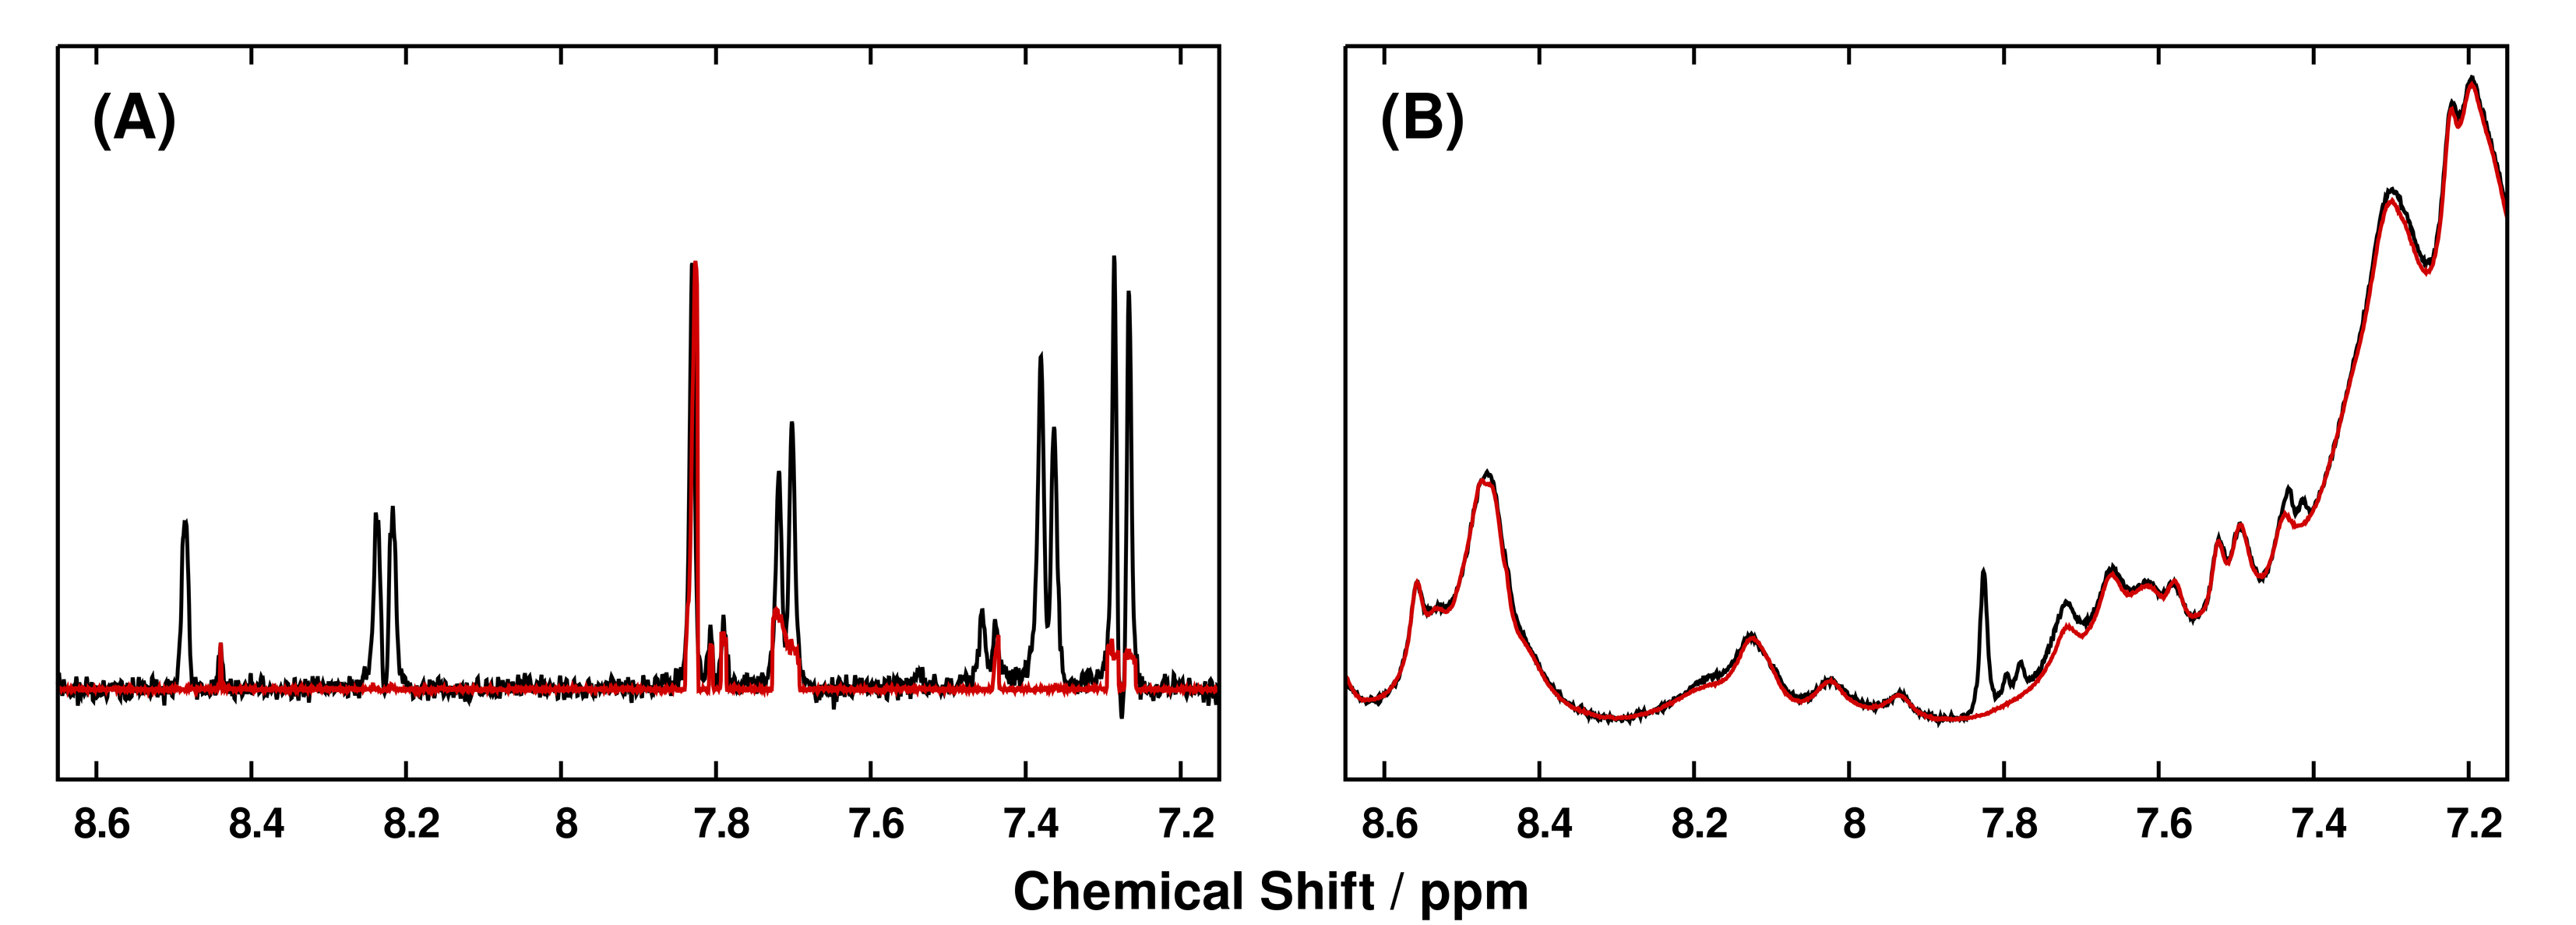
\includegraphics[width=6.5in]{figs/ussr/02-ussrfit.png}
\caption
      [Statistical Baseline Removal from a Screen Spectrum.]{
  {\bf Statistical Baseline Removal from a Screen Spectrum.}
  \\
  An example spectral remodeling result of tolazamide, dimethyl
  4-methoxyisophthalate, 1,7-dimethylxanthine and oxolinic acid in the
  presence of BSA, showing ({\bf A}) the free ligand spectrum (black) and
  the remodeled spectrum (red) resulting from removing the statistical
  baseline (red) from the screen spectrum (black) in ({\bf B}). The remodeled
  pseudospectrum readily indicates that several peaks from dimethyl
  4-methoxyisophthalate have broadened into the baseline due to interaction
  with BSA.
}
\end{figure}

\subsection{Statistical Hit Determination}

\begin{doublespace}
For each peak in each remodeled spectrum from USSR, a $K_D$ was computed based
on the intensity ratio between free and remodeled ligand signals. First, in the
limit of fast exchange between free and bound ligand states relative to the NMR
timescale, the fraction of bound ligand ($f_B$) was computed:
\begin{equation}
f_B =
 \left( \frac{I_F}{I_B} - 1 \right)
 \left( \frac{v_B}{v_F} - 1 \right)^{-1}
\end{equation}
where $I_F$ and $I_B$ are the intensities of free and remodeled (bound) ligand
signals, and $v_F$ and $v_B$ are the estimated NMR line widths of the free and
remodeled ligand signals, respectively \cite{shortridge:jcomb2008}. This
fast-exchange assumption may be safely regarded as valid in most
high-throughput 1D \hnmr{} NMR protein-ligand affinity screening experiments
\cite{lepre:chemrev2004}, where the width and intensity of each ligand signal
is a population-weighted sum of its values in the free and bound states.
Without any assumptions about relative concentrations of ligand and protein,
the fraction of bound ligand is related to the total protein concentration
$[P]_T$, total ligand concentration $[L]_T$ and $K_D$ via the following
equation \cite{shortridge:jcomb2008}:
\begin{equation}
f_B = \left[
  1 + \frac{2 K_D}{
    ([P]_T - [L]_T - K_D) + \sqrt{([P]_T - [L]_T - K_D)^2 + 4 K_D [P]_T}
  }
\right]^{-1}
\end{equation}

The solution of the above equation for $K_D$ yields the following result:
\begin{equation}
K_D = \frac{(f_B - 1)(f_B [L]_T - [P]_T)}{f_B}
\end{equation}
which was used to computed per-peak $K_D$ values for each remodeled spectrum
$\mathbf{r}_n$. Finally, the per-peak $K_D$ values were used to compute sample
mean and standard deviation $K_D$ values for each ligand. Hit detection was
accomplished by comparing per-ligand mean and standard deviation $K_D$ values
against a threshold via a Student's $t$-test, where a resulting $p$ value less
than a predefined significant $p$ value was reported as binding.
\end{doublespace}

\begin{figure}[ht!]
\includegraphics[width=6.5in]{figs/ussr/03-ussrfail.png}
\caption
      [Failed Baseline Removal due to Phase Errors.]{
  {\bf Failed Baseline Removal due to Phase Errors.}
  \\
  Example of a failed USSR result, highlighting the impact of phase error
  during computation and subtraction of the statistical baseline from a screen
  spectrum. Remodeled peaks ({\bf A}, red) upfield of 4.0 ppm are in fact not
  true signals, but were generated due to a phase-induced discrepancy between
  the statistical baseline ({\bf B}, red) and the screen spectrum
  ({\bf B}, black).
}
\end{figure}

\subsection{Analysis of Dataset Size}

\begin{doublespace}
A small simulation study was conducted to assess the quality of USSR
statistical baseline estimates over a range of sample sizes (number of spectral
pairs). For sizes from 2 to 116, the BSA dataset was randomly subsampled,
without replacement, to produce a smaller dataset. For each resultant dataset,
the statistical baseline was estimated, and its Pearson correlation to the true
statistical baseline was computed and stored. Over all numbers of spectral
pairs in the simulation, the median baseline correlations were computed, and
are reported in Figure 7.4.
\end{doublespace}

\begin{SCfigure}
\includegraphics[width=3.5in]{figs/ussr/04-blcorr.png}
\caption
      [Impact of Dataset Size on USSR Statistical Baselines.]{
  {\bf Impact of Dataset Size on USSR Statistical Baselines.}
  \\
  Correlation between statistical baselines from bootstrap-subsampled datasets
  of varying size and the original statistical baseline computed from the
  complete BSA dataset. Lines indicate median correlations, and shaded regions
  indicate confidence regions of plus or minus one standard deviation,
  estimated using median absolute deviation. Blue lines and shaded regions
  indicate values from subsampling the PSC normalized dataset, and red lines
  and shaded regions indicate values from subsampling the uncorrected dataset.
}
\end{SCfigure}

\section{Results}

\begin{doublespace}
From the USSR analysis of ligand binding to BSA, 43 compounds were classified
as hits from the library of 456 compounds. All classified hits were determined
to bind BSA with at least 1.0 mM affinity ($K_D \le 0.001$ $\mu$M) at a
statistical confidence level of 99\%. A summary of the hits, along with their
estimated $K_D$ and $p$ valunes, is provided in Table 7.3. Comparison of
results from both PSC-corrected and uncorrected USSR datasets reveals that the
use of PSC normalization prior to USSR modeling greatly reduces the effective
positive rate of statistical hit determination: 195 hits were identified from
the PSC-uncorrected spectra. Closer examination of hits identified without PSC
correction indicates that USSR failed to fully subtract the statistical
baseline from the screen spectra (e.g. Figure 7.3), resulting in residual
baseline intensity passing into equation 7.2 during $K_D$ calculation and hit
determination. In short, the use of PSC normalization prior to USSR enables
more effective baseline subtraction by decreasing both dilution- and
phase-related protein baseline intensity variation in collected \hnmr{} NMR
spectra (Figure 7.5). Baseline estimates obtained by collecting a spectrum of
pure protein will suffer from the same phase-induced variation, which would
also increase the false positive rate during hit determination. The introduced
combination of PSC and USSR provides a more reliable means of baseline
identification, without the need for collection of a free protein reference
spectrum.
\end{doublespace}

\begin{SCfigure}
\includegraphics[width=3.5in]{figs/ussr/05-rsd.png}
\caption
      [Impact of PSC on USSR Statistical Baselines.]{
  {\bf Impact of PSC on USSR Statistical Baselines.}
  \\
  Relative standard deviations (RSDs) of the statistical baselines computed
  before (red) and after (black) phase-scatter correction, which substantially
  decreases inter-sample variability of the protein baseline signals.
}
\end{SCfigure}

\begin{doublespace}
Cursory analysis of the robustness of the USSR statistical
baseline during random subsampling of the BSA dataset indicated that the
PSC/USSR methodology can reliably operate at very low dataset sizes
(i.e. 10--20 spectral pairs). Pearson correlations between true and subsampled
baselines did not appreciably decrease even after harsh subsampling
(Figure 7.3), and correlations computed from PSC-normalized data maintained
significantly higher values than those from non-normalized data. While it
would be possible to obtain a statistical baseline from fewer than ten spectral
pairs, this is not recommended, as it will decrease the effectiveness of the
Bonferroni-corected $t$-test that USSR performs during remodeling. Therefore,
as a general rule of thumb, PSC/USSR analyses may be performed on
high-throughput screening datasets having as few as ten spectral pairs, and
higher sample sizes only serve to further increase the reliability of remodeled
results.
\end{doublespace}

\section{Discussion and Conclusions}

\begin{doublespace}
While the saturation transfer difference (STD) NMR experiment
\cite{mayer:jacs2001} is a popular choice for ligand-based NMR affinity
screens, a 1D \hnmr{} NMR spectrum requires only a few seconds to acquire,
making it an ideal choice for high-throughput screening. STD experiments
require significantly longer acquisition times (upwards of hours) in order
to acquire difference spectra with sufficient signal-to-noise to reduce false
negatives. A particular strength of STD is the minimal amount of protein
needed per experiment, making it practical to screen a reasonably large
chemical library (upwards of thousands of compounds) with only a few
milligrams of protein. Through a judicious choice of protein and ligand
concentrations coupled with the use of cryoprobes and high magnetic fields,
it is also possible to minimize protein requirements in 1D \hnmr{}
line-broadening screens. While STD experiments still tend to require less
protein than line-broadening experiments, the higher false positive rate of
STD screening easily negates any advantages of minimal protein usage. This
high false positive rate arises due to the tendency of STD experiments to
emphasize weak binding affinities commonly encountered during aggregation
and nonspecific binding \cite{harner:jbnmr2013,lepre:menz2011}.
\\\\
NMR line-broadening experiments take advantage of the molecular-weight
dependence of $T_2$ relaxation and the resultant measurable difference in
line-widths between proteins and the compounds in a screening library
\cite{hajduk:jacs1997}. Upon binding a protein target, the \hnmr{} NMR
resonances of a compound will broaden significantly or even disappear.
In principal, this spectral broadening is easily observable and binding is
readily identified. In practice, background signals from the protein can
confound the data analysis. This background interference increases with the
size and concentration of the protein and leads to an increase in false
negative rates. Apparent line-width differences between free and bound
ligands \emph{also} increase with protein size and concentration, making the
optimal experimental conditions for NMR line-broadening screens exactly the
same conditions which confound manual interpretation. Clearly, the ability to
accurately remove the protein background from an NMR line-broadening experiment
will improve both the utility and reliability of the technique, especially at
relatively high protein-ligand concentration ratios where binding is more
apparent.
\\\\
By removing interfering protein baseline signals, USSR provides a
straightforward means of visually or computationally analzing screening
results. In fact, the outcome of applying the USSR method to an extremely
challenging and atypical test case is rather dramatic: an NMR line-broadening
screen of BSA against a chemical library of 456 compounds identified 43
binders, despite the BSA background signals completely obscuring the ligand
spectral features. An example screening result of tolazamide, dimethyl
4-methoxyisophthalate, 1,7-dimethylxanthine and oxolinic acid against BSA is
illustrated in Figure 7.2. Removal of the interfering protein statistical
baseline from the screen spectrum (Figure 7.2B) yielded a high-quality
pseudo-spectrum of the ligand mixture in the presence of BSA. Overlaying the
remodeled NMR spectrum with the free ligand mixture spectrum indicated that
the two spectra were essentially identical for the non-binding ligands
(Figure 7.2A). Only dimethyl 4-methoxyisophthalate, which binds BSA, exhibited
any difference after remodeling. The USSR method of baseline estimation and
subtraction is expected to perform equally well under any conditions where a
common, highly reproducible spectral feature exists within a dataset. The
presented application of PSC/USSR to high-throughput protein-ligand affinity
screening is but one example of its potential uses.
\\\\
However, reliable identification of the protein baseline from screening data
requires highly reproducible sample preparation, data collection and
processing. The last of these requirements is met by the use of phase-scatter
correction prior to remodeling, which brings protein baselines from all spectra
into closer agreement with each other and minimizes the number of false hits
identified during analysis. It is important to note that PSC is only an
effective pre-treatment for USSR when protein baseline signals are of
comparable intensity to ligand signals. PSC normalization is designed to
maximize statistical agreements \emph{between} spectra by phase and
normalization correction, and its use of the $L_2$ norm as a criterion for
`agreement' implies that higher-intensity features will be preferentially
corrected. Thus, PSC achieves the best results prior to USSR when protein
signals are a major spectral component, as is the case when protein-ligand
concentration ratios are near or greater than unity. In effect, the combined
use of PSC and USSR expands the range of protein-ligand concentration ratios
which may be probed by \hnmr{} line-broadening experiments for the purposes
of high-throughput screening.
\\\\
Finally, it cannot be under-emphasized that the single-point $K_D$ computations
employed by USSR during statistical hit determination are only
order-of-magnitude estimates of the true dissociation rates, and can carry
significant systematic and random errors. In particular, the fraction of bound
ligand -- and by extension, the dissociation constant -- depends exquisitely
on the estimated free and bound ligand linewidths, $v_F$ and $v_B$. Thus, any
imprecision in the linewidth estimates will propagate into a systematic bias in
the final dissociation constants. If required, verification of initial hits may
be achieved to higher accuracy via multiple-point estimation of the $K_D$
through linear or nonlinear least squares \cite{shortridge:jcomb2008}.
\\\\
An implementation of the USSR algorithm is available in open-source GNU Octave
code as a part of the MVAPACK toolbox \cite{worley:acscb2014}.
\end{doublespace}

\begin{table}[h!]
\caption{Results of the USSR Analysis of Ligand Binding to BSA.}
\begin{center}
\begin{tabular}{l | l l}
  \hline
  {\bf Compound} & {\bf $K_D$ (nM)} & {\bf $p$} \\
  \hline
  Thiamine hydrochloride                    & 0.143 & $\le 10^{-6}$ \\
  5-azacytidine                             & 0.072 & $\le 10^{-6}$ \\
  Nadolol                                   & 0.142 & $\le 10^{-6}$ \\
  N-succinyl-Ala-Ala-Pro-Phe p-nitroanilide & 0.090 & $\le 10^{-6}$ \\
  Timolol maleate                           & 0.092 & $\le 10^{-6}$ \\
  5-phenylvaleric acid                      & 0.000 & $\le 10^{-6}$ \\
  Astemizole                                & 0.000 & $\le 10^{-6}$ \\
  Leflunomide                               & 0.041 & $\le 10^{-6}$ \\
  Gliotoxin                                 & 0.061 & $\le 10^{-6}$ \\
  2-aminofluorene                           & 0.141 & 0.000001 \\
  Mordant orange 1                          & 0.162 & 0.000020 \\
  Indomethacin                              & 0.239 & 0.000027 \\
  Diminazene aceturate                      & 0.186 & 0.000034 \\
  Flavanone                                 & 0.188 & 0.000065 \\
  (-)-arctigenin                            & 0.200 & 0.000101 \\
  Meclofenamic acid sodium salt             & 0.154 & 0.000188 \\
  2-acetamidophenol                         & 0.198 & 0.000202 \\
  Bromocresol green                         & 0.198 & 0.000266 \\
  Mycophenolic acid                         & 0.203 & 0.000341 \\
  7-deazaguanine                            & 0.213 & 0.000466 \\
  Camptothecin                              & 0.183 & 0.000468 \\
  Flavone                                   & 0.208 & 0.000582 \\
  Naproxen                                  & 0.211 & 0.000653 \\
  2,6-diisopropylphenol                     & 0.220 & 0.000816 \\
  Z-L-phenylalanine                         & 0.230 & 0.001076 \\
  Cromolyn sodium salt                      & 0.226 & 0.001080 \\
  Methotrexate, (+)-ametthopterin           & 0.237 & 0.001106 \\
  Cinoxacin                                 & 0.231 & 0.001224 \\
  Dimethyl 4-methoxyisophthalate            & 0.218 & 0.001315 \\
  8-methoxypsoralen                         & 0.237 & 0.002242 \\
  L-ornithine hydrochloride                 & 0.337 & 0.002326 \\
  Aminophylline hydrate                     & 0.246 & 0.002633 \\
  Captopril                                 & 0.277 & 0.002781 \\
  Ebselen                                   & 0.246 & 0.002854 \\
  2-aminophenol                             & 0.394 & 0.003476 \\
  Myristic acid                             & 0.271 & 0.004925 \\
  Sulindac sulfide                          & 0.269 & 0.005659 \\
  Phenylpyruvic acid                        & 0.282 & 0.006867 \\
  Diclofenac sodium salt                    & 0.284 & 0.007310 \\
  Prednisolone                              & 0.286 & 0.007693 \\
  Alaproclate hydrochloride                 & 0.281 & 0.007706 \\
  Phenylmethanesulfonyl fluoride            & 0.265 & 0.008433 \\
  Methyl 4-hydroxyphenylacetate             & 0.286 & 0.008845
\end{tabular}
\end{center}
\end{table}

\pagebreak
\bibliographystyle{abbrv}
\bibliography{bworley}

